\section{Introduction}
\begin{frame}{Theta-Curves}
	\begin{itemize}
		\item A \term{theta-curve} $T$ is a graph embedded in $S^3$,
		which consists of two vertices $v_1$, $v_2$
		and three edges $e_1$, $e_2$, $e_3$,
		such that each edge joins the vertices.
		\item A \term{constituent knot $T_{ij}$}, $1 \le i < j \le 3$, is a subgraph of $T$
		that consists of two vertices $v_1$, $v_2$ and two edges $e_i$, $e_j$.
		
		\item Theta-curves are roughly classified by comparing the triples of constituent knots.
		
		\item A theta-curve is said to be \term{trivial} if it can be embedded in a 2-sphere in $S^3$.

		$$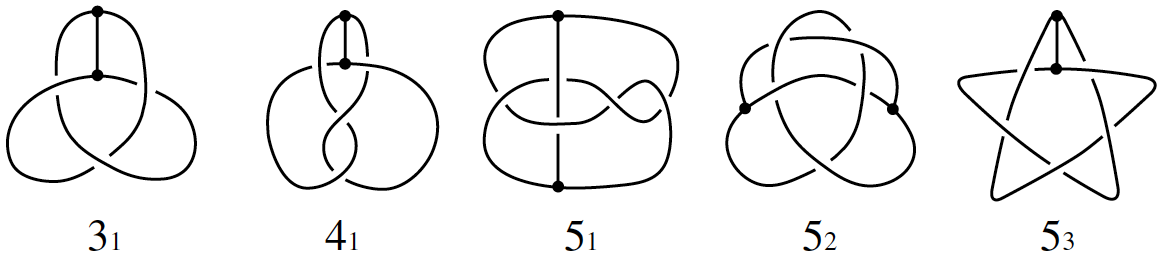
\includegraphics[width=.8\linewidth]{theta_exe.png}$$
	\end{itemize}
\end{frame}

\begin{frame}{Handcuff Graphs}
	\begin{itemize}
		\item \term{Handcuff graph} is the graph which consists of two loops and an edge jointing the vertices of each loop.
	\end{itemize}

	$$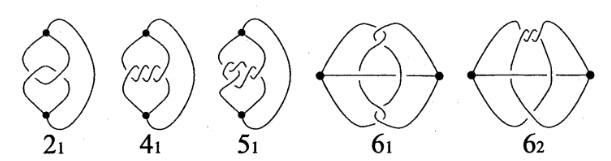
\includegraphics[width=.8\linewidth]{handcufflist.png}$$
\end{frame}

\begin{frame}{Reidemaister Moves for Theta-Curves and Handcuff Graphs}
	\medskip
	\begin{enumerate}
		\item[\mybf{I.}] \quad\raisebox{-15pt}{
\includegraphics[width=36pt,height=36pt]{y101}} \quad $\longleftrightarrow$ \quad \raisebox{-15pt}{
\includegraphics[width=36pt,height=36pt]{y103}} \quad $\longleftrightarrow$ \quad \raisebox{-15pt}{
\includegraphics[width=36pt,height=36pt]{y102}}\medskip
		\item[\mybf{II.}] \quad\raisebox{-15pt}{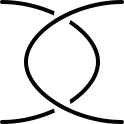
\includegraphics[width=36pt,height=36pt]{y111}} \quad $\longleftrightarrow$ \quad \raisebox{-15pt}{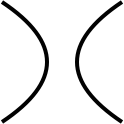
\includegraphics[width=36pt,height=36pt]{y93}} \quad $\longleftrightarrow$ \quad \raisebox{-15pt}{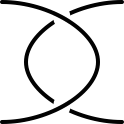
\includegraphics[width=36pt,height=36pt]{y112}}\medskip
		\item[\mybf{III.}] \quad\raisebox{-15pt}{
\includegraphics[width=36pt,height=36pt]{r31}} \quad $\longleftrightarrow$ \quad \raisebox{-15pt}{
\includegraphics[width=36pt,height=36pt]{r32}} \qquad\qquad\raisebox{-15pt}{
\includegraphics[width=36pt,height=36pt]{y121}} \quad $\longleftrightarrow$ \quad \raisebox{-15pt}{
\includegraphics[width=36pt,height=36pt]{y122}}\medskip
		\item[\mybf{IV.}] \quad\raisebox{-15pt}{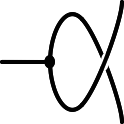
\includegraphics[width=36pt,height=36pt]{y141}} \quad $\longleftrightarrow$ \quad \raisebox{-15pt}{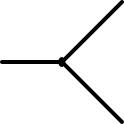
\includegraphics[width=36pt,height=36pt]{y143}} \quad $\longleftrightarrow$ \quad \raisebox{-15pt}{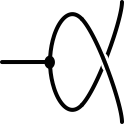
\includegraphics[width=36pt,height=36pt]{y142}}\medskip
		\item[\mybf{V.}] \quad\raisebox{-15pt}{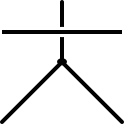
\includegraphics[width=36pt,height=36pt]{y131}} \quad $\longleftrightarrow$ \quad \raisebox{-15pt}{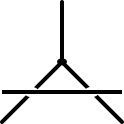
\includegraphics[width=36pt,height=36pt]{y132}} \qquad\qquad\raisebox{-15pt}{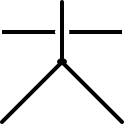
\includegraphics[width=36pt,height=36pt]{y133}} \quad $\longleftrightarrow$ \quad \raisebox{-15pt}{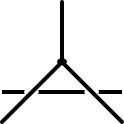
\includegraphics[width=36pt,height=36pt]{y134}}
	\end{enumerate}
\end{frame}

\begin{frame}{Arc Index}
    \begin{itemize}
        \item \term{Arc presentation} is an open-book decomposition of $\mathbb{R}^3$ which has open half-planes as pages and the standard z-axis as the binding axis.
        \item \term{Arc index}, is the minimal number of pages among all possible arc presentations of graph.
        \item This arc presentation with the minimal number of pages is \term{minimal arc presentation}.
    \end{itemize}
\end{frame}

\begin{frame}{Arc Index}
    \centering
    \begin{tabu}{X[c]X[c]X[c]}
        \raisebox{-1cm}{
\includegraphics[height=2cm]{Trefoilimage.png}} &
        \raisebox{-1.8cm}{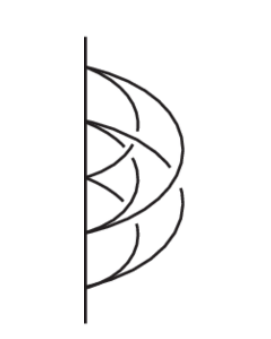
\includegraphics[height=3.6cm]{trefoil arc presentation.png}} &
        \raisebox{-1cm}{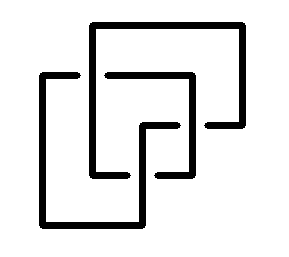
\includegraphics[height=2cm]{trefoil_grid.png}} \\
        Trefoil & Open Book & Grid Diagram
    \end{tabu}

\end{frame}


\begin{frame}{Arc Index}
    \centering
    \begin{tabu}{X[c]X[c]X[c]}
        \raisebox{-1cm}{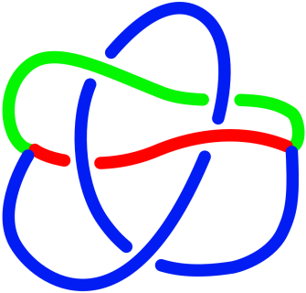
\includegraphics[height=2cm]{theta52.png}} &
        \raisebox{-1.8cm}{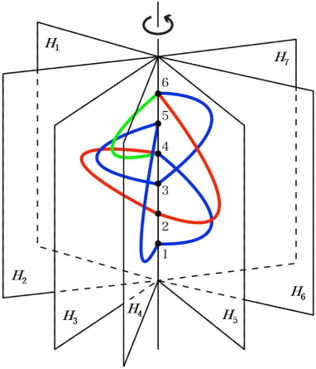
\includegraphics[height=3.6cm]{openbook.png}} &
        \raisebox{-1cm}{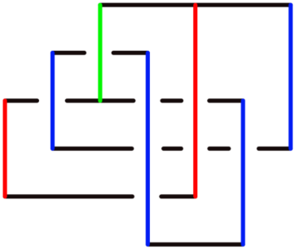
\includegraphics[height=2cm]{grid.png}} \\
        $\theta_{5,2}$ & Open Book & Grid Diagram
    \end{tabu}
\end{frame}


\begin{frame}{Arc Index}
    \centering
    \begin{tabu}{X[c]X[c]X[c]}
        \raisebox{-1cm}{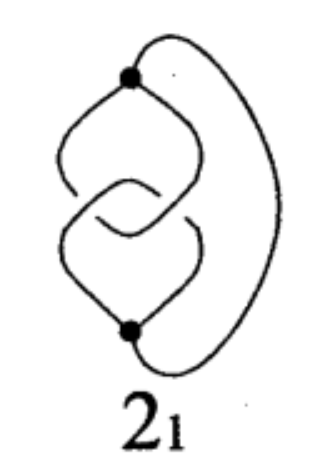
\includegraphics[height=2cm]{handcuff.png}} &
        \raisebox{-1.8cm}{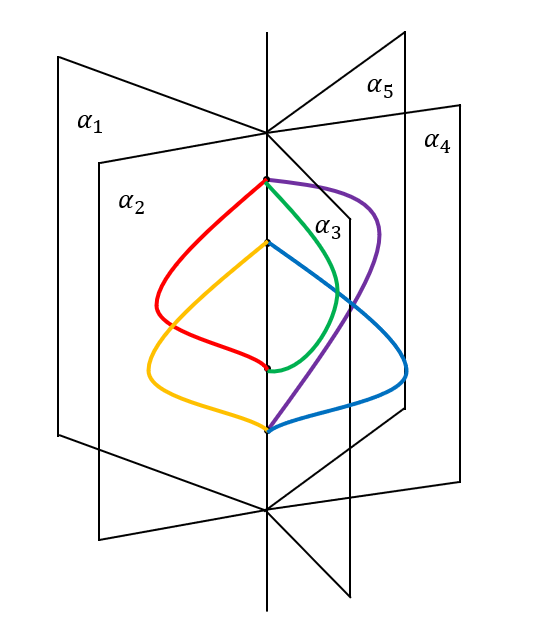
\includegraphics[height=3.6cm]{handcuff_openbook.png}} &
        \raisebox{-1cm}{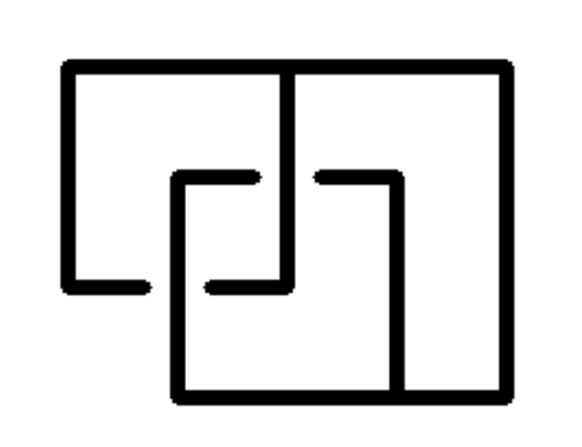
\includegraphics[height=2cm]{handcuff grid diagram.png}} \\
        $\Phi_{2,1}$ & Open Book & Grid Diagram
    \end{tabu}
\end{frame}

\begin{frame}{Grid Diagram}
	\begin{itemize}
		\item The \term{grid diagram} of a theta-curve or handcuff graph is a diagram of vertical strands and one less number of horizontal strands.
		\item At every crossing the vertical strand crosses over the horizontal strand and no two horizontal segments are co‐linear and no two vertical segments are co‐linear.
	\end{itemize}
\begin{figure}
    \centerline{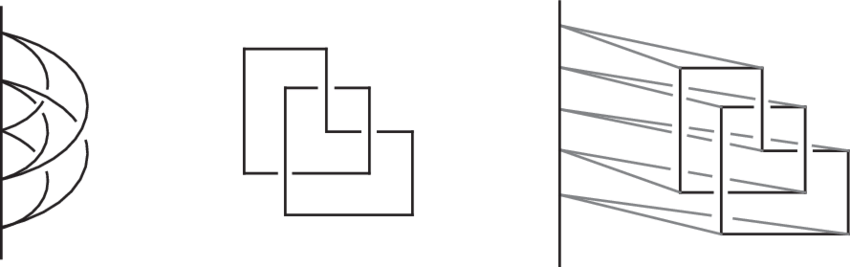
\includegraphics[width=0.75\linewidth]{../figs/An_arc_presentation_and_a_grid_diagram_of_the_knot.png}}
\end{figure}
\end{frame}

\begin{frame}{Cromwell Matrix}
	\begin{itemize}
		\item The \term{Cromwell matrix} of a knot is an $n \times n$ binary matrix each of whose rows and columns has exactly two 1s.
    \end{itemize}
    \centering
    \begin{tabu}{X[c]X[c]X[c]}
        \raisebox{-1cm}{
\includegraphics[height=2cm]{Trefoilimage.png}} &
        \raisebox{-1.8cm}{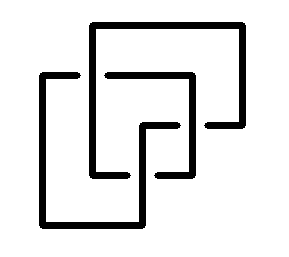
\includegraphics[height=3.6cm]{trefoil_grid.png}} &
        \raisebox{-1cm}{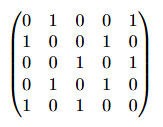
\includegraphics[height=2cm]{trefoil_cromwell.png}} \\
        Trefoil & Grid Diagram & Cromwell Matrix
    \end{tabu}
\end{frame}

\begin{frame}{Arc Presentation of the Theta-Curve and Handcuff Graph}
	\begin{thm}
    Arc presentations exist for every theta-curve and handcuff graph. 
	\end{thm}
	\mypf
    \begin{center}
    \begin{tabu}{c c c}
        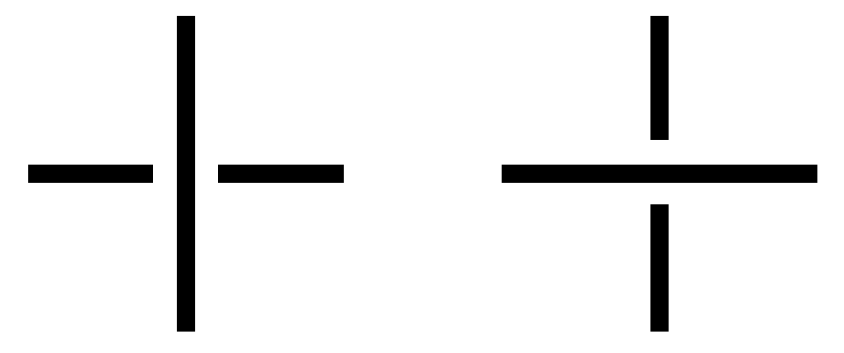
\includegraphics[width=0.4\linewidth]{figure/crossings.png} &
        \raisebox{1cm}{$\xmapsto{}$} &
        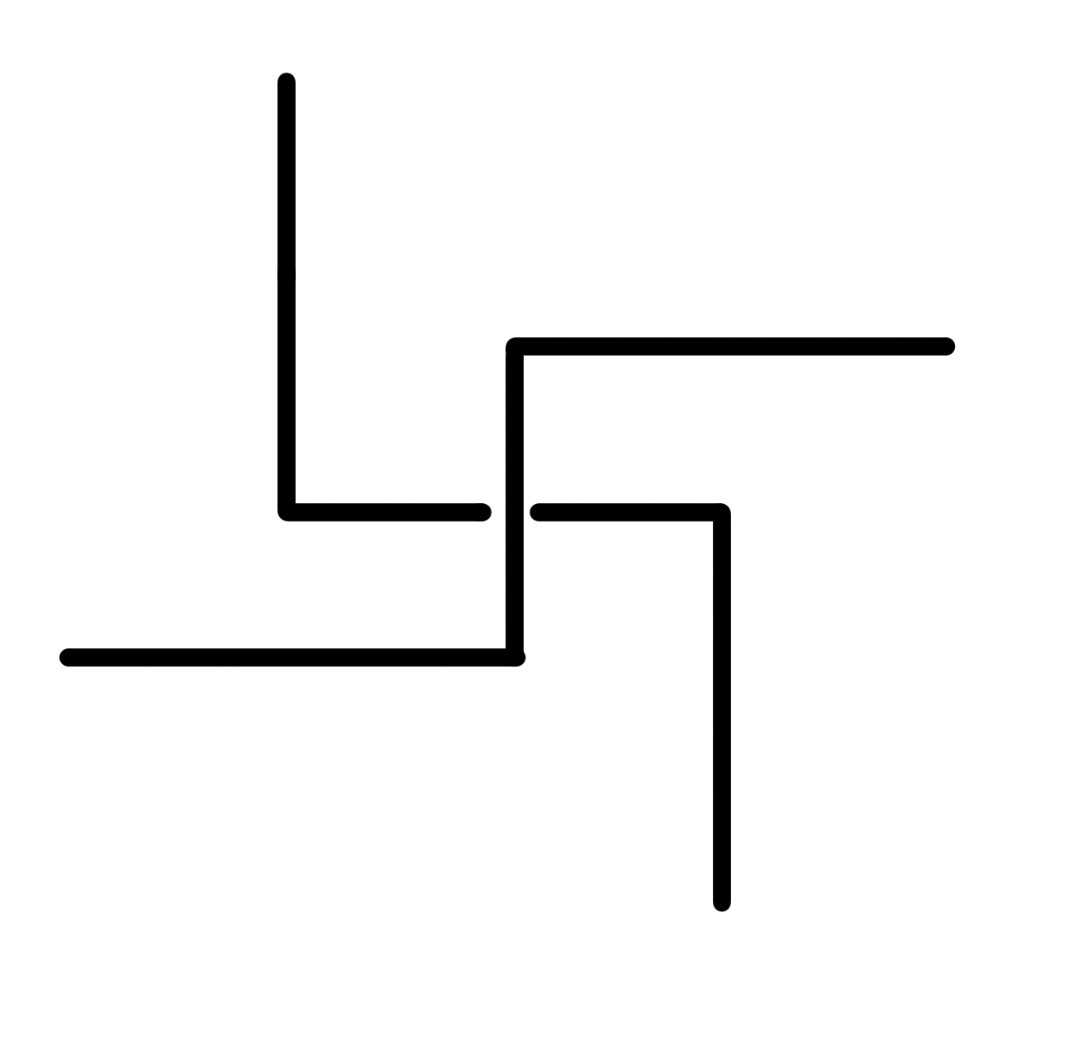
\includegraphics[width=0.2\linewidth]{changed_crossing.jpg}
    \end{tabu}
    \end{center}
\end{frame}

